\documentclass[10pt,conference]{IEEEtran}
\IEEEoverridecommandlockouts

\usepackage{cite}
\usepackage{amsmath,amssymb,amsfonts}
\usepackage{graphicx}
\usepackage{textcomp}
\usepackage{xcolor}
\usepackage{booktabs}
\usepackage{url}
\usepackage{balance}
\usepackage{tikz}
\usepackage{pgfplots}
\usetikzlibrary{positioning,shapes.geometric,arrows.meta,fit,backgrounds}
\pgfplotsset{compat=1.18}

\setlength{\textfloatsep}{6pt plus 2pt minus 2pt}
\setlength{\floatsep}{6pt plus 2pt minus 2pt}
\setlength{\intextsep}{6pt plus 2pt minus 2pt}

\newcommand{\brb}{\textsc{BR-Bench}}
\newcommand{\brs}{\textsc{BR-Seeded}}

\begin{document}

\title{BlastRadius: Predicting, Triaging and Repairing\\the Tests a Code Change Breaks}

\author{
\IEEEauthorblockN{Deepanshu\IEEEauthorrefmark{1}, Sanskriti Singh\IEEEauthorrefmark{1}, Prisha Vadhavkar\IEEEauthorrefmark{1}, Dr.~Yoga Raja C A\IEEEauthorrefmark{2}}
\IEEEauthorblockA{\IEEEauthorrefmark{1}School of Computer Science Engineering and Information Systems\\
Vellore Institute of Technology, Vellore, Tamil Nadu, India\\
\{deepanshu.2023, sanskriti.singh2023, prisha.vadhavkar2023\}@vitstudent.ac.in}
\IEEEauthorblockA{\IEEEauthorrefmark{2}Assistant Professor Sr. Grade 1, Department of Information Technology\\
School of Computer Science Engineering and Information Systems\\
Vellore Institute of Technology, Vellore, Tamil Nadu, India\\
yogaraja.ca@vit.ac.in}
}

\maketitle

\begin{abstract}
When a pull request fails in continuous integration (CI), a developer wants to know three things: which tests the change is likely to break, whether a failing test is really their fault, and how to fix it. We study all three on real data. First we build \brb{}, a dataset that links pull-request changes in GitHub Actions to the individual tests they caused to fail, with failures inherited from the base branch and same-commit flips removed. The strict split holds 4,168 fault-revealing labels on 762 changes from 37 Java and Python repositories. On it, file co-change, a label common in change impact analysis, recalls 4.64\% of the failing test files at $k=10$, while past failure frequency recalls 39.44\%. We then use the data to build BlastRadius, a four-stage assistant that predicts, runs, triages and repairs. Measured with the metrics of our base paper, predictive test selection at Meta, a learned ranker catches 56.8\% of failing test files at a selection rate of 0.10 and needs 0.764 of the candidates to reach a test recall of 0.95, which Meta reports at under 0.33 on private data; on the same data it reaches Recall@10 of 0.525 against 0.522 for the strongest published baseline, a difference that is not significant. A failure classifier clears inherited and flaky failures while wrongly clearing 1.37\% of real regressions, at low recall. In a pre-registered repair experiment on 70 seeded bugs, giving an open-weight model the diff raised the number of patches that pass the full test suite from 33 to 50 (exact McNemar $p=0.00076$), and a second model showed the same effect (19 to 41). We report the negative results as plainly as the positive ones.
\end{abstract}

\begin{IEEEkeywords}
continuous integration, regression testing, test selection, failure triage, program repair, mining software repositories
\end{IEEEkeywords}

\section{Introduction}

Given a code change, which tests will it break? The question is old, and most of the answers in the literature are indirect. Change impact analysis predicts which program entities are edited together, usually from version history~\cite{huang2022change}. Regression test selection computes, from static or dynamic dependencies, a safe superset of the tests a change may affect, as in Ekstazi~\cite{gligoric2015practical} and STARTS~\cite{legunsen2017starts}, and recent work tries to make that superset smaller without losing safety~\cite{liu2023more}. Neither records which tests actually failed. Predictive test selection at Meta~\cite{machalica2019predictive} learns from real failures, and later work on learned prioritisation does the same~\cite{pan2022test,yaraghi2022scalable}, but much of the industrial evidence rests on data that are not public, and the open benchmarks work at the level of the build job rather than the change~\cite{mattis2020rtptorrent}.

This matters in two ways. A method can look good against co-change and still be poor at finding the tests that break, and so far there has been no public way to check. And a developer whose pull request goes red has more than one problem. Some failing tests were already failing on the target branch; some flip on the same commit; and the real ones still have to be fixed. A CI server such as Jenkins runs the tests and reports the verdicts, but it does not say which failures belong to the change or what to do about them.

We approach the problem from the data side. Let a pull-request run have head commit $H$, and let $B$ be the commit of the branch it targets. A test is \emph{fault-revealing} for the run if it fails at $H$, does not fail in a run of the same workflow at (or near) $B$, and gives the same verdict in every run of one commit. We mine such tests from GitHub Actions logs and release them as \brb{}. On top of the data we build BlastRadius, an assistant with four stages: it \emph{predicts} which test files are at risk, \emph{runs} them first, \emph{triages} each failure as the change's own, inherited or flaky, and proposes a \emph{repair} that is kept only if the full test suite passes.

We ask five research questions.
\begin{itemize}
\item \textbf{RQ1.} How well do cheap proxies (co-change, the changed files, failure history) find the fault-revealing test files of a change?
\item \textbf{RQ2.} Does a learned ranker, trained on \brb{}, rank failing test files higher than published baselines?
\item \textbf{RQ3.} Can past CI data separate a change's own failures from inherited and flaky ones without clearing real regressions?
\item \textbf{RQ4.} Does knowing the change help a language model repair a failing build?
\item \textbf{RQ5.} Is the gain in RQ4 only better retrieval of code?
\end{itemize}

\textit{Summary of results.}
\begin{itemize}
\item \brb{} has 762 strict instances with 4,168 labels on 2,466 distinct tests; 94.29\% of test identifiers bind to a source file (Section~\ref{sec:data}).
\item Co-change recalls 4.64\% of fault-revealing test files at $k=10$, failure history 39.44\% (Section~\ref{sec:rq1}).
\item In the base paper's metrics, the ranker needs 76.4\% of candidate tests for a test recall of 0.95, against under 33\% reported at Meta on private data (Section~\ref{sec:rq2a}).
\item The learned ranker ties the strongest baseline (0.525 vs.\ 0.522, Holm-adjusted $p=0.382$); our own target for the ranker is therefore not met (Section~\ref{sec:rq2}).
\item Triage is a trade-off on a small sample: the best model clears 14.35\% of inherited and flaky failures and wrongly clears 1.37\% of real ones (Section~\ref{sec:rq3}).
\item Change-aware repair beats log-only repair on both models, and retrieval over the whole repository does not close the gap (Sections~\ref{sec:rq4} and~\ref{sec:rq5}).
\end{itemize}

The rest of the paper is organised as follows. Section~\ref{sec:related} places the work. Section~\ref{sec:data} describes how \brb{} is built, and Section~\ref{sec:system} the four stages of BlastRadius. Section~\ref{sec:setup} gives the experimental setup and Section~\ref{sec:results} the results. We discuss them in Section~\ref{sec:discussion} and list threats in Section~\ref{sec:threats}.

\section{Related Work}
\label{sec:related}

\textit{Test selection and prioritisation.} Regression test selection aims at safety, that is, no affected test is skipped. Ekstazi~\cite{gligoric2015practical} tracks file dependencies at run time and STARTS~\cite{legunsen2017starts} computes class dependencies statically; Liu et al.~\cite{liu2023more} make selection more precise by reasoning about which changes alter semantics. Learned prioritisation takes the opposite view and ranks tests by the chance that they fail. The predictive test selection system of Machalica et al.~\cite{machalica2019predictive}, trained on test outcomes at Meta, is the closest industrial precedent for our ranker and the main motivation for building an open dataset of the same kind. Pan et al.~\cite{pan2022test} review machine-learning approaches to selection and prioritisation, and Yaraghi et al.~\cite{yaraghi2022scalable} show that a large set of CI features can be computed at scale. Bertolino et al.~\cite{bertolino2020learning} compare learning-to-rank with other learners on CI data, Elsner et al.~\cite{elsner2021empirically} show that information already available in CI (test history, changed files, test age) goes a long way, and Zhao et al.~\cite{zhao2023revisiting} revisit machine-learning prioritisation for CI on a common set of subjects. Peng et al.~\cite{peng2020empirically} revisit information-retrieval prioritisation, which matches the text of a change against the text of tests. We use the last three lines of work as baselines. Other studies predict outcomes one level up: whether a test suite will fail~\cite{pan2021continuous} or whether a build will fail~\cite{sun2024ravenbuild}, and Jin and Servant~\cite{jin2021what} compare strategies that make CI cheaper.

\textit{Datasets.} RTPTorrent~\cite{mattis2020rtptorrent} records Travis CI build jobs of Java projects for prioritisation research; its unit is the job, not a pull-request diff. GHALogs~\cite{moriconi2025ghalogs} archives a large number of GitHub Actions logs but leaves them unparsed. GitBug-Actions~\cite{saavedra2024gitbug} uses GitHub Actions to build reproducible bug-fix benchmarks, and SWE-bench~\cite{jimenez2024swebench} turns GitHub issues into repair tasks. None of them links a single diff to the tests that the diff broke after inherited and flaky failures are removed.

\textit{Flakiness and triage.} A test is flaky if its verdict changes while the code does not. DeFlaker~\cite{bell2018deflaker} detects such tests by checking whether a failing test covered the latest change. Parry et al.~\cite{parry2021survey} survey the topic, Gruber et al.~\cite{gruber2021empirical} study flaky tests in Python projects, and Flakify~\cite{fatima2023flakify} predicts flakiness from test code with a language model. Closer to triage, Lampel et al.~\cite{lampel2021oranges} classify intermittent job failures at Mozilla, Olewicki et al.~\cite{olewicki2022brown} detect builds that fail for reasons unrelated to the change, and Henderson et al.~\cite{henderson2023flake} make culprit finding at Google aware of flaky tests. Our flake filter is simpler and uses only what CI logs show: a test that both passes and fails on one commit.

\textit{Program repair with language models.} Hou et al.~\cite{hou2024large} survey language models in software engineering. For repair, Xia et al.~\cite{xia2023automated} and Jiang et al.~\cite{jiang2023impact} measure what pre-trained models can fix, ChatRepair~\cite{xia2024automated} feeds test results back to the model in a conversation, and InferFix~\cite{jin2023inferfix} adds retrieved examples to the prompt, an instance of retrieval-augmented generation~\cite{lewis2020retrieval}. Agentless~\cite{xia2025agentless} and AutoCodeRover~\cite{zhang2024autocoderover} first localise a fault and then ask for a patch. Our repair stage follows the same pattern. What we test is narrower: whether telling the model which code the change touched makes repair more likely, under a fixed acceptance rule.

\section{\brb{}: Data Collection and Labelling}
\label{sec:data}

\begin{figure}[t]
\centering
\resizebox{\columnwidth}{!}{%
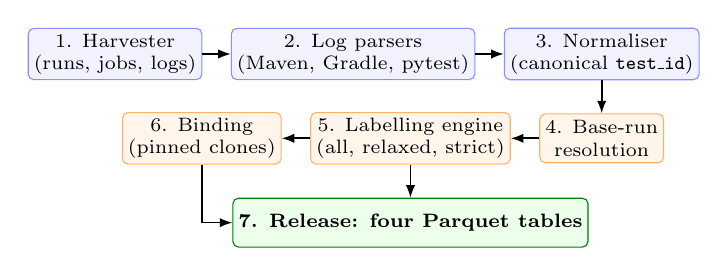
\begin{tikzpicture}[
  node distance=0.42cm and 0.36cm,
  every text node part/.style={align=center},
  box/.style={draw, rectangle, rounded corners=2pt, minimum height=0.62cm, minimum width=1.15cm, font=\scriptsize, inner sep=2pt},
  proc/.style={box, fill=blue!5, draw=blue!45},
  filt/.style={box, fill=orange!8, draw=orange!60},
  res/.style={box, fill=green!8, draw=green!50!black, font=\scriptsize\bfseries},
  arr/.style={-{Latex[length=1.6mm]}, semithick}
]
  \node[proc] (harvest) {1. Harvester\\(runs, jobs, logs)};
  \node[proc, right=of harvest] (parse) {2. Log parsers\\(Maven, Gradle, pytest)};
  \node[proc, right=of parse] (norm) {3. Normaliser\\(canonical \texttt{test\_id})};
  \node[filt, below=of norm] (base) {4. Base-run\\resolution};
  \node[filt, left=of base] (label) {5. Labelling engine\\(all, relaxed, strict)};
  \node[filt, left=of label] (bind) {6. Binding\\(pinned clones)};
  \node[res, below=of label] (release) {7. Release: four Parquet tables};
  \draw[arr] (harvest) -- (parse);
  \draw[arr] (parse) -- (norm);
  \draw[arr] (norm) -- (base);
  \draw[arr] (base) -- (label);
  \draw[arr] (label) -- (bind);
  \draw[arr] (bind) |- (release);
  \draw[arr] (label) -- (release);
\end{tikzpicture}}
\caption{The seven stages that turn GitHub Actions runs into \brb{}.}
\label{fig:pipeline}
\end{figure}

The data pipeline has seven stages (Fig.~\ref{fig:pipeline}). Every stage is deterministic, and no language model takes part in it.

\textit{Sampling and harvesting.} Candidate repositories come from the SEART search tool~\cite{dabic2021sampling}. Of 3,671 exported repositories, 2,646 had at least 100 GitHub Actions runs in the previous 90 days, and 2,333 of these had a workflow that runs tests rather than only linting or deployment. We drew 300 of them, balanced between Java and Python. The harvester ran from 8 to 29 August 2026 and reached 77 repositories with 175,038 runs; the instance table covers 76 of them and 165,349 runs. For each run it stored run and job metadata, check-run annotations and the raw logs. The time window was not a free choice. GitHub Actions deletes logs after 90 days, and at the last capture 4,458 of 13,422 failed runs in the corpus (33.21\%) were already older than that.

\textit{Parsing and identifiers.} Line parsers read Maven Surefire and Failsafe, Gradle and pytest output, and emit a verdict and, where printed, a duration for each test. Every test then gets one canonical identifier, the \texttt{test\_id}: \texttt{fully.qualified.Class\#method} for Java and \texttt{path::name} for Python. All later stages join on this key.

\textit{Base-run resolution.} A test that fails at $H$ may already fail at $B$. We therefore look for a base run, a run of the same workflow that shows which tests failed without the change, in a fixed order: a successful run at $B$ whose log shows tests running (\texttt{exact\_green}), another run at $B$ (\texttt{exact}), a run on an ancestor of $B$ at most 10 commits away (\texttt{ancestor}), or the latest earlier run on the target branch (\texttt{branch\_prior}). If none exists the status is \texttt{no\_base} and the run yields no label. An empty failure set is never read as a green base. Of the 12,581 failed runs, 5,520 (43.88\%) end as \texttt{no\_base}.

\textit{Labels.} We write $F_H$ for the tests that fail in a head run, $F_B$ for those that fail in its base run, and $X$ for same-SHA flips (tests that fail in some, but not all, runs of one workflow on one commit). Then
\begin{equation}
T_{\text{reveal}} = (F_H \setminus F_B) \setminus X .
\label{eq:reveal}
\end{equation}
The engine emits three nested splits: \texttt{all} keeps every head failure in a run with a known base, \texttt{relaxed} removes $F_B$, and \texttt{strict} also removes $X$. Flips are rare; they occur in 62 of 11,557 (commit, workflow, test) groups (0.54\%) and remove 46 of 4,214 relaxed labels.

\textit{Binding.} Each \texttt{test\_id} is bound to a test source file in a clone pinned to a recorded commit. A unique match on the fully qualified class name has confidence 1.0, a match on the bare class name 0.5.

\begin{table}[t]
\caption{Attrition of Runs and the Resulting Splits}
\label{tab:funnel}
\centering
\scriptsize
\setlength{\tabcolsep}{3pt}
\resizebox{\columnwidth}{!}{%
\begin{tabular}{@{}lrr@{}}
\toprule
\textbf{Stage} & \textbf{Runs} & \textbf{\% of previous} \\
\midrule
Discovered & 165,349 & -- \\
Failed & 12,581 & 7.61\% \\
Failed-job log on disk & 6,586 & 52.35\% \\
At least one parsed failing test & 1,774 & 26.94\% \\
Base run resolved & 1,348 & 75.99\% \\
Base failure set known & 897 & 66.54\% \\
At least one strict label & 762 & 84.95\% \\
\midrule
\textbf{Split} & \textbf{Instances / labels / tests} & \textbf{Java share} \\
\midrule
\texttt{all} & 897 / 4,384 / 2,500 & 85.5\% \\
\texttt{relaxed} & 770 / 4,214 / 2,484 & 83.9\% \\
\texttt{strict} & 762 / 4,168 / 2,466 & 83.7\% \\
\bottomrule
\end{tabular}}
\end{table}

\textit{The resulting data.} Table~\ref{tab:funnel} follows the runs through the pipeline. Most losses occur at the logs: only about half of the failed runs still had a failed-job log, and only 1,774 contained a failing test that the parsers recognise. The strict split has 762 instances, 4,168 labels and 2,466 distinct tests from 37 repositories. Java dominates, with 35 of the 37 repositories and 3,855 of the 4,168 labels. Of 5,985 distinct (repository, \texttt{test\_id}) pairs, 5,643 (94.29\%) bind to a file, 3,820 (63.83\%) at full confidence; 178 are absent from the pinned tree and 164 match several files. The release consists of four Parquet tables (\texttt{instances}, \texttt{outcomes}, \texttt{cochange} and \texttt{failure\_messages}, with 165,349, 12,766, 175,204 and 3,490 rows), with author logins replaced by keyed hashes and a datasheet in the form of Gebru et al.~\cite{gebru2021datasheets}.

\begin{table}[t]
\caption{\brb{} Next to the Public CI Datasets It Builds On}
\label{tab:datasets}
\centering
\scriptsize
\setlength{\tabcolsep}{3pt}
\resizebox{\columnwidth}{!}{%
\begin{tabular}{@{}llll@{}}
\toprule
\textbf{Property} & \textbf{RTPTorrent~\cite{mattis2020rtptorrent}} & \textbf{GHALogs~\cite{moriconi2025ghalogs}} & \textbf{\brb{}} \\
\midrule
CI system & Travis CI & GitHub Actions & GitHub Actions \\
Unit & build job & workflow run (raw log) & pull-request run with its diff \\
Per-test verdicts & yes & no (unparsed) & yes, parsed \\
Base-branch failures removed & no & no & yes \\
Flaky failures removed & no & no & yes (same-commit flips) \\
Tests bound to source files & no & no & yes (94.29\%) \\
Languages & Java & many & Java, Python \\
\bottomrule
\end{tabular}}
\end{table}

\textit{Comparison with existing datasets.} Table~\ref{tab:datasets} sets \brb{} beside the two public CI datasets closest to it. RTPTorrent~\cite{mattis2020rtptorrent} gives per-test verdicts but counts every failure of a job, including those already present on the target branch; GHALogs~\cite{moriconi2025ghalogs} is far larger but keeps the logs as text. \brb{} is smaller than both. What it adds is the label: each failing test is tied to one pull-request diff, and failures that the diff did not cause are subtracted before release.

\section{The BlastRadius System}
\label{sec:system}

\begin{figure}[t]
\centering
\resizebox{\columnwidth}{!}{%
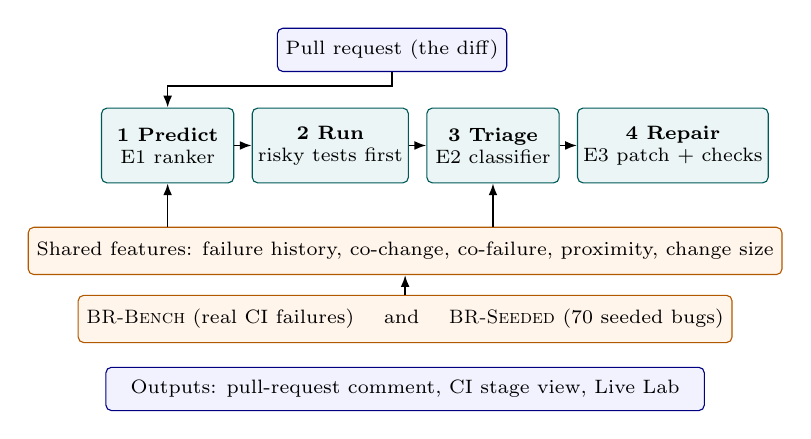
\begin{tikzpicture}[
  node distance=0.30cm and 0.22cm,
  every text node part/.style={align=center},
  st/.style={draw=teal!70!black, fill=teal!8, rounded corners=2pt, minimum width=1.68cm, minimum height=0.95cm, font=\scriptsize, inner sep=2pt},
  dat/.style={draw=orange!70!black, fill=orange!8, rounded corners=2pt, minimum height=0.6cm, font=\scriptsize, inner sep=3pt},
  outb/.style={draw=blue!50!black, fill=blue!5, rounded corners=2pt, minimum height=0.55cm, font=\scriptsize, inner sep=3pt},
  arr/.style={-{Latex[length=1.5mm]}, semithick}
]
  \node[outb] (pr) {Pull request (the diff)};
  \node[st, below=0.45cm of pr, xshift=-2.85cm] (p) {\textbf{1 Predict}\\E1 ranker};
  \node[st, right=of p] (r) {\textbf{2 Run}\\risky tests first};
  \node[st, right=of r] (t) {\textbf{3 Triage}\\E2 classifier};
  \node[st, right=of t] (f) {\textbf{4 Repair}\\E3 patch + checks};
  \draw[arr] (pr.south) -- ++(0,-0.18) -| (p.north);
  \draw[arr] (p) -- (r); \draw[arr] (r) -- (t); \draw[arr] (t) -- (f);
  \node[dat, below=0.55cm of r, xshift=0.95cm, minimum width=7.6cm] (feat) {Shared features: failure history, co-change, co-failure, proximity, change size};
  \node[dat, below=0.25cm of feat, minimum width=7.6cm] (data) {\brb{} (real CI failures) \quad and \quad \brs{} (70 seeded bugs)};
  \draw[arr] (feat.north -| p.south) -- (p.south);
  \draw[arr] (feat.north -| t.south) -- (t.south);
  \draw[arr] (data) -- (feat);
  \node[outb, below=0.30cm of data, minimum width=7.6cm] (ui) {Outputs: pull-request comment, CI stage view, Live Lab};
\end{tikzpicture}}
\caption{The four stages of BlastRadius and the data behind them. Stages 1 and 3 are trained and tested on \brb{}; stage 4 is tested on \brs{}.}
\label{fig:system}
\end{figure}

BlastRadius takes a pull request and passes it through four stages (Fig.~\ref{fig:system}). The prediction and triage stages read one shared feature layer, and every feature of a run uses only events that happened strictly before the run started.

\textit{Predict.} For each candidate test file of the repository, a LightGBM ranker with a LambdaRank objective scores the risk that the file fails. Its 24 features come in five families: failure history of the file (6), co-change between the file and the changed files (5), co-failure with other tests (2), proximity of the file to the changed files (5), and size and kind of the change (6).

\textit{Run.} The test files are run in the predicted order, so that the first failure appears early. Inside a file, tests are ordered by their distance to the changed code in the graph.

\textit{Triage.} Each failing (run, test) pair is classified as \emph{mine} (caused by the change), \emph{inherited} (already failing on the base) or \emph{flaky}. The classifier sees only the history before the run, such as earlier failures of the test on the branch and whether the same failure message was seen before. The dangerous error is to clear a real regression, so we report that error separately; the decision threshold is chosen on validation data to maximise F1 for the not-mine class.

\textit{Repair.} The repair agent retrieves at most three code chunks, asks a model for a patch, applies it with a strict applier and runs five checks: the patch applies, the code compiles, the failing tests pass, the full suite passes, and no file outside the allowed set is edited. A patch is accepted only if all five pass. This is the only stage that calls a language model, and every reply is cached so that the experiment replays offline.

\textit{Outputs.} The results reach the developer as a comment on the pull request and as a stage view in CI. For demonstration we also built the Live Lab, a web interface in which a reviewer picks a repository, injects a bug and watches the four stages run on it. Nothing the Live Lab produces enters the numbers below.

\section{Experimental Setup}
\label{sec:setup}

\textit{Comparison with the reference papers.} Our base paper is predictive test selection at Meta~\cite{machalica2019predictive}, and every result below is set against the paper it builds on, on that paper's own metric. Two kinds of comparison are kept apart. A \emph{same-data} comparison runs a published method on \brb{} next to ours; a \emph{published-number} comparison places our result next to a number reported on other data, which shows where we stand but is not a contest. For a selection strategy $s$, let $F(d)$ be the tests that failed on change $d$ and $S(d)$ those that $s$ selected. The base paper defines
{\small
\begin{align}
\mathit{TestRecall}(s) &= \textstyle\sum_d |S(d)\cap F(d)| \,/\, \sum_d |F(d)|, \\
\mathit{ChangeRecall}(s) &= |\{d : S(d)\cap F(d)\neq\emptyset\}| \,/\, |\{d : F(d)\neq\emptyset\}|, \\
\mathit{SelectionRate}(s) &= \textstyle\sum_d |S(d)| \,/\, \sum_d |\mathit{Candidates}(d)|,
\end{align}
}
and reports $\mathit{TestRecall}>0.95$ and $\mathit{ChangeRecall}>0.999$ at $\mathit{SelectionRate}<0.33$, where the candidates are the tests that depend on the change in the build graph, more than 1,000 per change. Cutting our ranked list at a rate $x$ gives a selection strategy with $\mathit{SelectionRate}=x$, so the three metrics apply directly; our candidates are all test files of the repository.

\textit{Splits.} For RQ2 and RQ3 we split the 734 usable strict instances chronologically by run start time, 60/20/20, into 440 training, 146 validation and 148 test instances. A random split would let the model see the future of a repository. We also run a leave-one-repository-out evaluation. The chronological test split happens to contain only Java instances.

\textit{RQ1.} Each proxy returns at most $k=10$ test files. Co-change (all) returns the files most often edited together with the changed files over the 365 days of commits before the run; co-change (test) keeps only conventional test files; the changeset baseline returns the changed files; failure history returns the test files with the most earlier strict labels. An audit found that an earlier version of this measurement looked into the future, and we fixed it before measuring: co-change is mined in a trailing window, and each strict label is counted once.

\textit{RQ2.} We compare the ranker with eight baselines: retest-all in alphabetical order (B0), random order over 20 seeds (B1), changed test files (B2), co-change support (B3), failure history (B4), BM25 over path tokens after Peng et al.~\cite{peng2020empirically} (B5), a history-only learning-to-rank model after Bertolino et al.~\cite{bertolino2020learning} (B6), and a model on readily available CI information after Elsner et al.~\cite{elsner2021empirically} (B7). The main metric is Recall@10 over the failing test files of an instance. We use the paired Wilcoxon signed-rank test with one Holm correction over a family of 10 comparisons, Cliff's $\delta$ for effect size, and a bootstrap with 10,000 resamples for confidence intervals. Before running the test we set ourselves a target: the ranker must beat the best baseline with adjusted $p<0.05$ and $|\delta|\geq 0.147$.

\textit{RQ3.} The positive class is \emph{not mine} (inherited or flaky), the failures a developer may stop investigating. We compare two rules, R-branch (the test failed in any of the previous three runs of the branch) and R-msg (the failure message was seen before), with logistic regression and LightGBM. Because the chronological test split has only 18 not-mine pairs, we report the pooled leave-one-repository-out result over all 4,384 pairs (216 not mine).

\textit{RQ4 and RQ5.} Real CI failures cannot be re-run on demand, so we built \brs{}: 70 tasks in four Python repositories (click 22, itsdangerous 22, markupsafe 19, shopcart 7). Each task applies one mutation operator to a function the test suite covers, so that at least one test fails, and adds two or three harmless edits in other files; the result plays the part of a pull request. A \emph{hard} variant adds four to six no-op edits inside functions the failing tests execute. The arms differ only in what the model is shown. R0 makes no repair. R1 sees the failure log and three chunks retrieved by BM25 over all functions of the repository. R2 sees the log and three chunks retrieved from the functions the diff touched. R3 is R2 with up to two further attempts that see the previous check results. We used two open-weight models, gpt-oss-120b and gpt-oss-20b~\cite{openai2025gptoss}, on the Groq free tier. The analysis plan was written and fixed before the main runs: the primary test is R2 against R1 on gpt-oss-120b, standard variant, by a one-sided exact McNemar test. For RQ5 we compare BM25, dense and hybrid retrieval (reciprocal rank fusion) over the whole repository with BM25 over the changed functions; this part was not pre-registered.

\section{Results}
\label{sec:results}

\begin{table*}[t]
\caption{Results at a Glance: Each Reference Paper, Its Reported Result and Ours}
\label{tab:glance}
\centering
\scriptsize
\setlength{\tabcolsep}{3pt}
\resizebox{\textwidth}{!}{%
\begin{tabular}{@{}llllll@{}}
\toprule
\textbf{Reference} & \textbf{Metric} & \textbf{Their result} & \textbf{Our result} & \textbf{Same data} & \textbf{Verdict} \\
\midrule
Machalica et al.~\cite{machalica2019predictive} (base) & share of tests for TestRecall 0.95 / ChangeRecall 0.999 & $<$0.33 / $<$0.33 (private) & 0.764 / 0.997 & no & lower \\
Elsner et al.~\cite{elsner2021empirically} & Recall@10; APFD; share of tests for 0.95 & -- & 0.525 vs 0.522; 0.852 vs 0.842; 0.764 vs 0.977 & yes & tie ($p=0.382$); better \\
Bertolino et al.~\cite{bertolino2020learning} & Recall@10; APFD & -- & 0.525 vs 0.477; 0.852 vs 0.791 & yes & higher, $p=0.223$ \\
Peng et al.~\cite{peng2020empirically} & Recall@10; APFD & -- & 0.525 vs 0.141; 0.852 vs 0.623 & yes & better, $p<0.001$ \\
Plyusnin et al.~\cite{plyusnin2025targeted} & TestRecall near 15\% of tests & 0.95 (private) & 0.568 at 10\%, 0.662 at 20\% & no & lower \\
Huang et al.~\cite{huang2022change} & co-change as impact label & ground truth & recalls 4.64\% of real failures & yes & weak label \\
RTPTorrent~\cite{mattis2020rtptorrent}, GHALogs~\cite{moriconi2025ghalogs} & label design & job verdicts; raw logs & diff-level, base and flakes removed & -- & different design (Table~\ref{tab:datasets}) \\
Ekstazi~\cite{gligoric2015practical}, STARTS~\cite{legunsen2017starts} & tests selected, one demo change & safe superset & reachability 272/297; first failure at 17 of 297 & yes & illustration only \\
Lampel et al.~\cite{lampel2021oranges} & precision / recall, ignorable failures & 73\% / 82\% & 37.6\% / 34.3\% & no & lower (4.9\% vs 67\% positives) \\
ChatRepair~\cite{xia2024automated}, Agentless~\cite{xia2025agentless} & bugs fixed; cost per fix & 48.1\%, 27.33\%; \$0.42, \$0.34 & 71.4\%; \$0.00042 & no & higher on easier bugs \\
CI-Bench~\cite{nabil2026cibench}, CI-Repair-Bench~\cite{muna2026cirepair} & CI failures repaired & 13--36\%; 7.9--18.9\% & 47.1\% log-only, 71.4\% change-aware & no & +24 points from the change \\
\bottomrule
\end{tabular}}
\end{table*}

Table~\ref{tab:glance} gathers every comparison. On the same data, our ranker ties the strongest published ranker on Recall@10 and needs fewer tests for high recall; against the base paper's private industrial numbers it is lower, for reasons Section~\ref{sec:rq2a} names; triage is more cautious than at Mozilla but less sensitive; and repair with the change in view succeeds far more often than without it, on bugs easier than those of the published repair benchmarks.

\subsection{RQ1: Cheap Proxies}
\label{sec:rq1}

\begin{figure}[t]
\centering
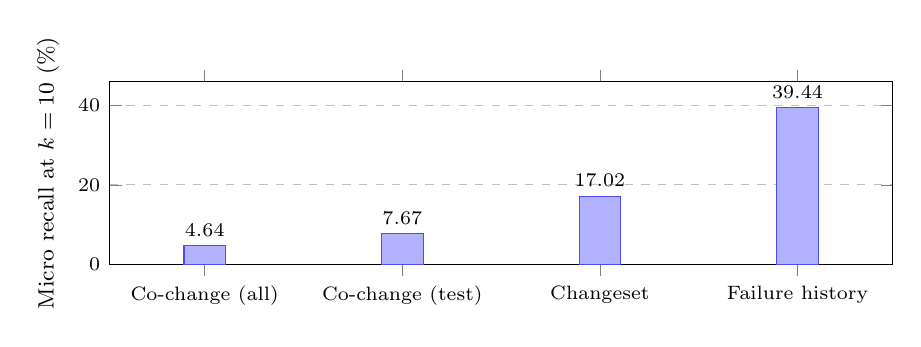
\begin{tikzpicture}
\begin{axis}[
    ybar, bar width=15pt, width=0.95\columnwidth, height=3.9cm,
    ymin=0, ymax=46,
    ylabel={Micro recall at $k=10$ (\%)},
    symbolic x coords={Co-change (all), Co-change (test), Changeset, Failure history},
    xtick=data, nodes near coords, nodes near coords align={vertical},
    every node near coord/.append style={font=\scriptsize},
    tick label style={font=\scriptsize}, label style={font=\footnotesize},
    ymajorgrids=true, grid style=dashed, enlarge x limits=0.16,
]
\addplot[fill=blue!30, draw=blue!70] coordinates {
    (Co-change (all), 4.64) (Co-change (test), 7.67) (Changeset, 17.02) (Failure history, 39.44)
};
\end{axis}
\end{tikzpicture}
\caption{RQ1: micro recall at $k=10$ of four proxies on the same 576 strict instances (1,316 fault-revealing test files).}
\label{fig:rq1}
\end{figure}

Of the 734 strict instances with a bound label, 576 have a non-empty co-change set (462 Java, 114 Python), and we score every proxy on exactly these, with 1,316 fault-revealing test files. Fig.~\ref{fig:rq1} shows the result. Co-change (all) finds 61 of the 1,316 files (4.64\%), co-change (test) 101 (7.67\%), the changed files 224 (17.02\%) and failure history 519 (39.44\%). The order stays the same when environment and timeout failures are removed. Co-change, then, is a poor label for the tests a change breaks. Failure history needs no analysis of the code at all, and it is the baseline any predictor has to beat.

\subsection{RQ2a: Comparison with the Base Paper}
\label{sec:rq2a}

\begin{table}[t]
\caption{Our Ranker in the Metrics of the Base Paper}
\label{tab:pts}
\centering
\scriptsize
\setlength{\tabcolsep}{2.5pt}
\resizebox{\columnwidth}{!}{%
\begin{tabular}{@{}lll@{}}
\toprule
\textbf{Quantity} & \textbf{Meta~\cite{machalica2019predictive}} & \textbf{Ours, \brb{}} \\
\midrule
Data & private monorepo & 148 changes, public Java repos \\
Candidates per change & $>$1,000 build-dependent tests & all test files, mean 924 \\
Model & GBDT classifier & GBDT (LightGBM) ranker \\
TestRecall at rate 0.10 / 0.20 / 0.50 & not reported & 0.568 / 0.662 / 0.834 \\
Rate for TestRecall $\geq$ 0.95 & $<$0.33 & 0.764 \\
Rate for ChangeRecall $\geq$ 0.999 & $<$0.33 & 0.997 \\
Same-data: rate for 0.95, Elsner et al. (B7) & -- & 0.977 \\
Same-data: rate for 0.95, failure history (B4) & -- & 0.806 \\
\bottomrule
\end{tabular}}
\end{table}

\begin{figure}[t]
\centering
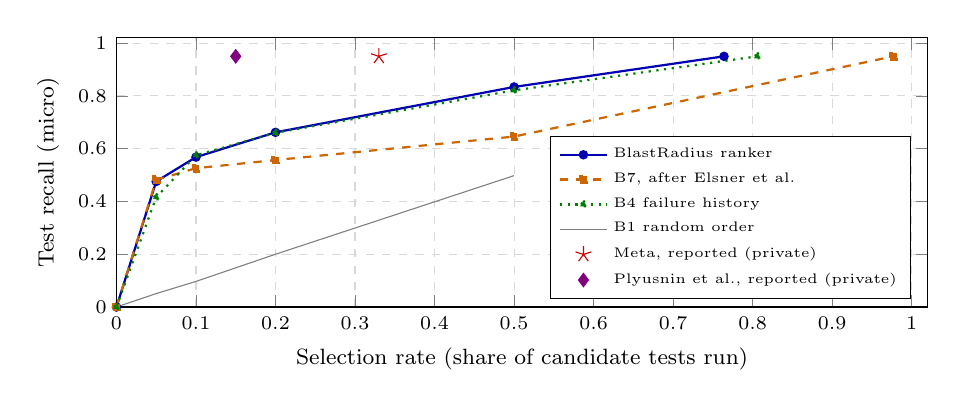
\begin{tikzpicture}
\begin{axis}[
    width=0.98\columnwidth, height=5.0cm,
    xmin=0, xmax=1.02, ymin=0, ymax=1.02,
    xlabel={Selection rate (share of candidate tests run)},
    ylabel={Test recall (micro)},
    tick label style={font=\scriptsize}, label style={font=\footnotesize},
    legend style={font=\tiny, at={(0.98,0.03)}, anchor=south east, cells={anchor=west}},
    grid=major, grid style={dashed, gray!30},
]
\addplot[thick, blue!70!black, mark=*, mark size=1.3pt] coordinates {(0,0) (0.05,0.476) (0.10,0.568) (0.20,0.662) (0.50,0.834) (0.764,0.95)};
\addlegendentry{BlastRadius ranker}
\addplot[thick, orange!80!black, dashed, mark=square*, mark size=1.2pt] coordinates {(0,0) (0.05,0.482) (0.10,0.526) (0.20,0.557) (0.50,0.646) (0.977,0.95)};
\addlegendentry{B7, after Elsner et al.}
\addplot[thick, green!50!black, dotted, mark=triangle*, mark size=1.4pt] coordinates {(0,0) (0.05,0.416) (0.10,0.575) (0.20,0.660) (0.50,0.821) (0.806,0.95)};
\addlegendentry{B4 failure history}
\addplot[gray, mark=none] coordinates {(0,0) (0.05,0.051) (0.10,0.097) (0.20,0.200) (0.50,0.498)};
\addlegendentry{B1 random order}
\addplot[only marks, mark=star, mark size=3pt, red!80!black] coordinates {(0.33,0.95)};
\addlegendentry{Meta, reported (private)}
\addplot[only marks, mark=diamond*, mark size=2.4pt, violet] coordinates {(0.15,0.95)};
\addlegendentry{Plyusnin et al., reported (private)}
\end{axis}
\end{tikzpicture}
\caption{Test recall against selection rate on the 148 test changes of \brb{}, with the operating points the base paper and Plyusnin et al.\ report on their own private data. The last point of each curve is the rate needed for a test recall of 0.95.}
\label{fig:pts}
\end{figure}

Table~\ref{tab:pts} and Fig.~\ref{fig:pts} set our ranker next to the base paper, with test recall pooled over all failing files as the base paper defines it. Selecting the top 10\% of candidate files catches 56.8\% of all failing files (73.5\% of a change's failing files on average), and the top half catches 83.4\%, against 49.8\% for random order. This is the behaviour the base paper describes, but not its level. Meta reports test recall above 0.95 at a third of its candidates; our ranker needs 76.4\% of the candidates to reach 0.95, and catching a failure in 99.9\% of faulty changes needs almost the whole suite (0.997), because in a few changes one failing file is ranked near the bottom. On the same data the ranker reaches 0.95 much earlier than Elsner et al.'s ranker (0.764 against 0.977) and a little earlier than failure history alone (0.806). The gap to Meta has identifiable causes: a candidate set already narrowed by the build graph, test targets rather than files, and months of dense history for every test. Other published operating points sit in between: Elsner et al.~\cite{elsner2021empirically} keep 90\% of failures while saving 84\% of test time on 23 projects, and Plyusnin et al.~\cite{plyusnin2025targeted} report recall 0.95 at 15\% of tests on industrial data. Like the base paper, which re-ran failing tests up to ten times, we remove flaky failures before training, because a model trained on flaky labels looks better than it is; on our test changes, counting flaky and inherited failures adds only 3 failing files (344 against 341), so test recall with and without flakes is essentially the same.

\subsection{RQ2b: Same-Data Comparison with Published Rankers}
\label{sec:rq2}

\begin{table}[t]
\caption{RQ2: Ranking Failing Test Files on the 148 Chronological Test Instances (Median 595 Candidate Files per Instance)}
\label{tab:e1}
\centering
\scriptsize
\setlength{\tabcolsep}{2.6pt}
\resizebox{\columnwidth}{!}{%
\begin{tabular}{@{}lrrrrr@{}}
\toprule
\textbf{Method} & \textbf{R@1} & \textbf{R@10} & \textbf{MAP} & \textbf{APFD} & \textbf{1st fail} \\
\midrule
B0 retest-all (alphabetical) & 0.081 & 0.089 & 0.097 & 0.469 & 551.1 \\
B1 random (20 seeds) & 0.003 & 0.029 & 0.020 & 0.490 & 429.9 \\
B2 changed test files & 0.132 & 0.227 & 0.182 & 0.560 & 444.1 \\
B3 co-change support & 0.047 & 0.144 & 0.085 & 0.497 & 500.7 \\
B4 failure history & 0.135 & 0.439 & 0.249 & 0.766 & 233.9 \\
B5 BM25 path tokens~\cite{peng2020empirically} & 0.024 & 0.141 & 0.080 & 0.623 & 349.5 \\
B6 history-only LTR~\cite{bertolino2020learning} & 0.235 & 0.477 & 0.341 & 0.791 & 229.3 \\
B7 readily-available LTR~\cite{elsner2021empirically} & 0.231 & 0.522 & 0.359 & 0.842 & \textbf{153.0} \\
\textbf{BlastRadius ranker} & \textbf{0.274} & \textbf{0.525} & \textbf{0.381} & \textbf{0.852} & 169.8 \\
\bottomrule
\end{tabular}}
\end{table}

Table~\ref{tab:e1} gives the main result. The ranker has the highest Recall@1, Recall@10, MAP and APFD, and it is clearly better than every simple baseline: against failure history (B4) its Recall@10 is 0.525 against 0.439 (Holm-adjusted $p=0.010$). Against the two learned baselines, however, the difference is within noise. Its Recall@10 of 0.525 (95\% CI $[0.447, 0.599]$) against 0.522 for B7 gives a Holm-adjusted $p=0.382$ and Cliff's $\delta=+0.030$, a negligible effect; against B6 the adjusted $p$ is 0.223. B7 also reaches the first failing file sooner on average (position 153.0 against 169.8). Our own target is therefore not met. On APFD, the metric Bertolino et al. and Peng et al. use, the ranker scores 0.852 against 0.842 for Elsner et al.'s ranker, 0.791 for Bertolino et al.'s and 0.623 for Peng et al.'s; the IR ranker is weak here because Java test file names often say little about the code they exercise.

The ablation shows where the signal lies. Removing the failure-history family lowers Recall@10 from 0.525 to 0.385 and removing the proximity family lowers it to 0.450; both drops exceed the variation over five seeds. Removing co-change changes it by $-0.007$, co-failure by $-0.001$ and change features by nothing, all within that variation. Co-change features add almost nothing once history and proximity are known, which agrees with RQ1. Training on the most recent 20\% of the training data already gives 0.467, and the full set 0.524. In the leave-one-repository-out evaluation, on the 12 repositories with at least 20 instances, the ranker beats both B4 and B5 on 9; on unicode-org/cldr failure history alone is much stronger (0.955 against 0.679).

\subsection{RQ3: Triage}
\label{sec:rq3}

\begin{table}[t]
\caption{RQ3: Triage, Pooled Leave-One-Repository-Out over 4,384 Failing Pairs (216 Not Mine, 4,168 Mine)}
\label{tab:e2}
\centering
\scriptsize
\setlength{\tabcolsep}{3pt}
\resizebox{\columnwidth}{!}{%
\begin{tabular}{@{}lrrr@{}}
\toprule
\textbf{Method} & \textbf{Not mine cleared} & \textbf{Mine wrongly cleared} & \textbf{F1} \\
\midrule
Blame all (everything is mine) & 0/216 (0.0\%) & 0/4,168 (0.00\%) & 0.000 \\
R-branch (failed in last 3 runs) & 145/216 (67.1\%) & 1,262/4,168 (30.28\%) & 0.179 \\
R-msg (message seen before) & 135/216 (62.5\%) & 848/4,168 (20.35\%) & 0.225 \\
Logistic regression & 74/216 (34.3\%) & 123/4,168 (2.95\%) & 0.358 \\
LightGBM & 31/216 (14.4\%) & 57/4,168 (1.37\%) & 0.204 \\
\bottomrule
\end{tabular}}
\end{table}

Table~\ref{tab:e2} shows the trade-off. The simple rules clear about two thirds of inherited and flaky failures, but they also tell the developer to ignore 20 to 30\% of real regressions, which makes them unusable. The learned models are far more careful. LightGBM wrongly clears 57 of 4,168 real failures (1.37\%) and logistic regression 123 (2.95\%), but they clear only 14.4\% and 34.3\% of the failures that could be ignored. On the chronological test split LightGBM clears 10 of 18 not-mine pairs while wrongly clearing 33 of 1,015, but 18 positives are too few to read much into. Triage on this data is a trade-off on a small sample, not a solved problem. The base rate explains part of it: only 216 of 4,384 failing pairs (4.9\%) are not the change's own. The closest published result is Lampel et al.~\cite{lampel2021oranges}, who classify intermittent job failures at Mozilla with 73\% precision and 82\% recall on average; in their data 67\% of failures were intermittent. Our logistic regression reaches 37.6\% precision and 34.3\% recall for the not-mine class. With positives this rare, high precision is hard to reach, and the rules that catch two thirds of them clear too many real regressions to be usable.

\subsection{RQ4: Change-Aware Repair}
\label{sec:rq4}

\begin{table}[t]
\caption{RQ4: Plausible Fixes (Full Test Suite Passes) on the 70 Standard \brs{} Tasks}
\label{tab:e3}
\centering
\scriptsize
\setlength{\tabcolsep}{2.8pt}
\resizebox{\columnwidth}{!}{%
\begin{tabular}{@{}llrrrr@{}}
\toprule
\textbf{Model} & \textbf{Arm} & \textbf{Plausible fix} & \textbf{95\% CI} & \textbf{Exact restore} & \textbf{Tokens} \\
\midrule
gpt-oss-120b & R1 log only & 33/70 & [0.36, 0.59] & 24/70 & 1,813 \\
 & R2 change-aware & 50/70 & [0.61, 0.81] & 43/70 & 1,369 \\
 & R3 R2 + retries & 55/70 & [0.69, 0.89] & 45/70 & 2,206 \\
\midrule
gpt-oss-20b & R1 log only & 19/70 & [0.17, 0.37] & 19/70 & 1,601 \\
 & R2 change-aware & 41/70 & [0.47, 0.70] & 39/70 & 1,386 \\
 & R3 R2 + retries & 48/70 & [0.57, 0.79] & 46/70 & 2,525 \\
\bottomrule
\end{tabular}}
\end{table}

Table~\ref{tab:e3} gives the plausible-fix rates; R0 fixes nothing by construction. The primary pre-registered test is supported. On gpt-oss-120b, R2 produced a patch that passes the full suite for 50 of 70 tasks and R1 for 33; R2 alone succeeded on 22 tasks and R1 alone on 5, and the one-sided exact McNemar test gives $p=0.00076$. The smaller model shows the same effect more strongly, 41 against 19 (25 against 3 discordant tasks, Holm-adjusted $p<10^{-4}$). R2 also used fewer tokens per task than R1, because the retrieved chunks are more to the point. Retries add a little more: R3 reaches 55 and 48 of 70. The gain of R3 over R2 is significant after correction for the smaller model ($p=0.031$) but not for the larger one ($p=0.094$).

Two observations limit the claim. A patch can pass the targeted tests and still break the suite; this happened for 3 of the R2 patches on each model, and the full-suite check rejected all of them. And seeded bugs are simpler than real ones, so these rates say what knowing the change adds, not how well the models repair real faults. The hard-variant runs are incomplete because of the free-tier quota (29 and 17 of 70 tasks so far), and we leave them out of the claim. We also note a negative side result: on these Python repositories, which have no failure history, ordering test files with the RQ2 ranker put the first failing file at mean position 10.91, later than alphabetical order (8.11).

\begin{table}[t]
\caption{Repair: Published Results on Their Own Benchmarks and Ours}
\label{tab:repaircmp}
\centering
\scriptsize
\setlength{\tabcolsep}{2.5pt}
\resizebox{\columnwidth}{!}{%
\begin{tabular}{@{}llrr@{}}
\toprule
\textbf{System} & \textbf{Benchmark} & \textbf{Fixed} & \textbf{Cost/fix} \\
\midrule
ChatRepair~\cite{xia2024automated} & Defects4J & 162/337 (48.1\%) & \$0.42 \\
Agentless~\cite{xia2025agentless} & SWE-bench Lite & 27.33\% & \$0.34$^{a}$ \\
CI-Bench tools~\cite{nabil2026cibench} & 100 BugSwarm failures & 13--36\% & -- \\
CI-Repair-Bench~\cite{muna2026cirepair} & 567 GHA failures & 7.9--18.9\%$^{b}$ & -- \\
Ours, R1 log only & \brs{} (70) & 33/70 (47.1\%) & \$0.00088$^{c}$ \\
\textbf{Ours, R2 change-aware} & \brs{} (70) & \textbf{50/70 (71.4\%)} & \$0.00042$^{c}$ \\
\bottomrule
\end{tabular}}
\\[2pt]{\scriptsize $^{a}$per issue; $^{b}$Pass@1; $^{c}$gpt-oss-120b at list price, USD 0 paid.}
\end{table}

\textit{Comparison with published repair systems.} Table~\ref{tab:repaircmp} places our rates next to published ones. Ours are higher, but they must not be read as better repair: seeded single-operator bugs in small libraries are far easier than Defects4J bugs, SWE-bench issues or real CI failures. What the comparison does show is the effect under test. Our log-only arm R1 receives the input of log-based CI repair tools, and fixes 47.1\%; the same model given the code the change touched fixes 71.4\% of the same tasks, at about a thousandth of a dollar per fix.

\subsection{RQ5: Is It Only Retrieval?}
\label{sec:rq5}

\begin{table}[t]
\caption{RQ5: Seeded Function Among the Top 3 Retrieved Chunks (70 Tasks per Variant, No Model Involved)}
\label{tab:rag}
\centering
\scriptsize
\setlength{\tabcolsep}{3pt}
\resizebox{\columnwidth}{!}{%
\begin{tabular}{@{}lrr@{}}
\toprule
\textbf{Retrieval mode} & \textbf{Standard} & \textbf{Hard} \\
\midrule
L1 BM25, whole repository (= R1) & 46/70 & 46/70 \\
L2 dense, whole repository & 21/70 & 21/70 \\
L3 hybrid (RRF), whole repository & 32/70 & 32/70 \\
L4 BM25, changed functions (= R2) & \textbf{69/70} & \textbf{63/70} \\
L5 hybrid, changed functions & \textbf{69/70} & 58/70 \\
\bottomrule
\end{tabular}}
\end{table}

If R2 wins only because it retrieves the right code, a better retriever over the whole repository should do as well. It does not (Table~\ref{tab:rag}). Hybrid retrieval over the whole repository finds the seeded function in 32 of 70 tasks, fewer than plain BM25 (46; Holm-adjusted $p=0.010$), while BM25 over the changed functions finds it in 69. On the standard variant part of this advantage holds by construction, since the seeded edit is inside the diff. The hard variant, which places no-op edits inside executed functions, removes some of it, and change-aware BM25 still finds the function in 63 of 70. Knowing the change helps more than a smarter search over code that does not know it.

\section{Discussion}
\label{sec:discussion}

The results have one common thread: in CI the past is a strong signal, and what the change touched is the next one. Failure history beats co-change by a wide margin (RQ1) and carries most of the ranker's strength (RQ2); the diff is what makes repair work (RQ4) and retrieval alone does not replace it (RQ5). Co-change, the label much impact-analysis research is built on, carries little information about failures.

Safe selection and learned ranking answer different questions, and one change from our Live Lab shows the difference. On a pull request to itsdangerous that flipped one comparison, 5 of 297 tests failed. Static class-level reachability in the style of STARTS~\cite{legunsen2017starts} selected 272 tests, almost the whole suite; per-test coverage, which needs an instrumented run first, selected 97 and caught all five; the ranker ran every test but reached the first failure at position 17, against 283 in alphabetical order. On a second recording with noisy decoy edits the ranker was slower than alphabetical order (99 against 45). One change proves nothing, and we do not count these figures as results, but they show why safety and early failure are separate goals.

A fair question is how this differs from what a CI server already does. Jenkins, or GitHub Actions on its own, runs every test and reports the verdicts. BlastRadius does not replace that. It orders the tests so that a failure tends to appear earlier, it tells the developer which failures are probably not theirs, and it proposes a patch that is accepted only when the whole suite passes. Each of these is measured against baselines, and two of the four stages do not yet beat the strongest of them. We report this, because a dataset that shows where methods fail is more useful than a predictor tuned until it appears to win.

\section{Threats to Validity}
\label{sec:threats}

\textit{Construct.} The labels are observational. We re-ran no test, so a label says that a test failed at the head and not at the base; it does not prove that the change caused the failure. Environment failures (89) and timeouts (112) remain in the strict split. The parsers score 46 of 46 and 30 of 30 on two fixture sets, but both guided their development; an independent holdout exists and has not yet been scored by a blind annotator.

\textit{Internal.} Every feature uses only data from before the run, and a leakage audit checks this. The E1 and E2 numbers, and all dataset numbers, regenerate offline with one command. The E3 numbers depend on recorded model replies, which we replay from a cache; a fresh run with the same model may differ.

\textit{External.} 35 of the 37 strict repositories are Java projects, the chronological test split is all Java, and a few active repositories contribute many instances. \brs{} uses four small Python repositories and five mutation operators. We did not reach our own target of 5,000 strict labels (4,168), and full-confidence binding (63.83\%) is below the 70\% we aimed for.

\section{Data Availability}

\brb{} is openly available on Zenodo under CC BY 4.0~\cite{brbench_data} (release v0.2, DOI 10.5281/zenodo.23688064; all versions, DOI 10.5281/zenodo.23250261). Release v0.2 keeps the rows of v0.1 and adds base-run, test-to-file binding and changeset fields. The code is released under the MIT licence and archived on Zenodo~\cite{brbench_code} (DOI 10.5281/zenodo.23250690). Rebuilding the labels from logs needs our raw log store, because most of the logs have since expired on GitHub.

\section{Conclusion}

We built \brb{}, a public dataset of the tests that pull requests really broke in GitHub Actions, and used it to measure four stages of CI assistance. Failure history is the signal to beat; co-change is a weak label for failures; a learned ranker matches the best published baseline but does not beat it; triage is still a trade-off; and telling a model what the change touched makes repair markedly more likely. Two questions stay open. How many of the labels would survive an isolated re-run? And can any signal drawn from the code add to failure history once both are measured on the same data? We hope \brb{} makes both questions easier to test.

\section*{Acknowledgment}
 No AI system takes part in data collection, labelling, the ranker, the triage models or the computation of their numbers. The repair experiment evaluates open-weight language models by design; their replies are recorded and replayed, and every reported number is regenerated by a script in the repository.

\balance
\begin{thebibliography}{99}

\bibitem{machalica2019predictive}
M.~Machalica, A.~Samylkin, M.~Porth, and S.~Chandra, ``Predictive test selection,'' in \emph{Proc. 41st Int. Conf. Softw. Eng.: Softw. Eng. Pract. (ICSE-SEIP)}, IEEE, 2019, pp. 91--100.

\bibitem{gligoric2015practical}
M.~Gligoric, L.~Eloussi, and D.~Marinov, ``Practical regression test selection with dynamic file dependencies,'' in \emph{Proc. Int. Symp. Softw. Test. Anal. (ISSTA)}, ACM, 2015, pp. 211--222.

\bibitem{legunsen2017starts}
O.~Legunsen, A.~Shi, and D.~Marinov, ``{STARTS}: {STAtic} regression test selection,'' in \emph{Proc. 32nd IEEE/ACM Int. Conf. Automated Softw. Eng. (ASE), Tool Demos}, IEEE, 2017, pp. 949--954.

\bibitem{bell2018deflaker}
J.~Bell, O.~Legunsen, M.~Hilton, L.~Eloussi, T.~Yung, and D.~Marinov, ``{DeFlaker}: Automatically detecting flaky tests,'' in \emph{Proc. 40th Int. Conf. Softw. Eng. (ICSE)}, ACM, 2018, pp. 433--444.

\bibitem{huang2022change}
Y.~Huang, J.~Jiang, X.~Luo, X.~Chen, Z.~Zheng, N.~Jia, and G.~Huang, ``Change-patterns mapping: A boosting way for change impact analysis,'' \emph{IEEE Trans. Softw. Eng.}, vol.~48, no.~7, pp. 2376--2398, 2022.

\bibitem{liu2023more}
Y.~Liu, J.~Zhang, P.~Nie, M.~Gligoric, and O.~Legunsen, ``More precise regression test selection via reasoning about semantics-modifying changes,'' in \emph{Proc. 32nd ACM SIGSOFT Int. Symp. Softw. Test. Anal. (ISSTA)}, 2023.

\bibitem{pan2022test}
R.~Pan, M.~Bagherzadeh, T.~A. Ghaleb, and L.~Briand, ``Test case selection and prioritization using machine learning: A systematic literature review,'' \emph{Empirical Softw. Eng.}, vol.~27, 2022.

\bibitem{yaraghi2022scalable}
A.~S. Yaraghi, M.~Bagherzadeh, N.~Kahani, and L.~Briand, ``Scalable and accurate test case prioritization in continuous integration contexts,'' \emph{IEEE Trans. Softw. Eng.}, 2022.

\bibitem{mattis2020rtptorrent}
T.~Mattis, P.~Rein, F.~D{\"u}rsch, and R.~Hirschfeld, ``{RTPTorrent}: An open-source dataset for evaluating regression test prioritization,'' in \emph{Proc. 17th Int. Conf. Mining Softw. Repos. (MSR)}, ACM, 2020, pp. 385--396.

\bibitem{bertolino2020learning}
A.~Bertolino, A.~Guerriero, B.~Miranda, R.~Pietrantuono, and S.~Russo, ``Learning-to-rank vs ranking-to-learn: Strategies for regression testing in continuous integration,'' in \emph{Proc. 42nd Int. Conf. Softw. Eng. (ICSE)}, ACM, 2020, pp. 1--12.

\bibitem{elsner2021empirically}
D.~Elsner, F.~Hauer, A.~Pretschner, and S.~Reimer, ``Empirically evaluating readily available information for regression test optimization in continuous integration,'' in \emph{Proc. 30th ACM SIGSOFT Int. Symp. Softw. Test. Anal. (ISSTA)}, ACM, 2021, pp. 491--504.

\bibitem{zhao2023revisiting}
Y.~Zhao, D.~Hao, and L.~Zhang, ``Revisiting machine learning based test case prioritization for continuous integration,'' in \emph{Proc. IEEE Int. Conf. Softw. Maint. Evol. (ICSME)}, 2023.

\bibitem{peng2020empirically}
Q.~Peng, A.~Shi, and L.~Zhang, ``Empirically revisiting and enhancing {IR}-based test-case prioritization,'' in \emph{Proc. 29th ACM SIGSOFT Int. Symp. Softw. Test. Anal. (ISSTA)}, ACM, 2020, pp. 324--336.

\bibitem{pan2021continuous}
C.~Pan and M.~Pradel, ``Continuous test suite failure prediction,'' in \emph{Proc. 30th ACM SIGSOFT Int. Symp. Softw. Test. Anal. (ISSTA)}, 2021.

\bibitem{sun2024ravenbuild}
G.~Sun, S.~Habchi, and S.~McIntosh, ``{RavenBuild}: Context, relevance, and dependency aware build outcome prediction,'' in \emph{Proc. ACM Int. Conf. Found. Softw. Eng. (FSE)}, 2024.

\bibitem{jin2021what}
X.~Jin and F.~Servant, ``What helped, and what did not? {An} evaluation of the strategies to improve continuous integration,'' in \emph{Proc. 43rd Int. Conf. Softw. Eng. (ICSE)}, 2021.

\bibitem{moriconi2025ghalogs}
F.~Moriconi, T.~Durieux, J.-R. Falleri, R.~Troncy, and A.~Francillon, ``{GHALogs}: Large-scale dataset of {GitHub} {Actions} runs,'' in \emph{Proc. 22nd Int. Conf. Mining Softw. Repos. (MSR)}, IEEE, 2025, pp. 669--673.

\bibitem{saavedra2024gitbug}
N.~Saavedra, A.~Silva, and M.~Monperrus, ``{GitBug-Actions}: Building reproducible bug-fix benchmarks with {GitHub} {Actions},'' in \emph{Proc. 46th Int. Conf. Softw. Eng. (ICSE), Demonstrations}, 2024.

\bibitem{jimenez2024swebench}
C.~E. Jimenez, J.~Yang, A.~Wettig, S.~Yao, K.~Pei, O.~Press, and K.~Narasimhan, ``{SWE-bench}: Can language models resolve real-world {GitHub} issues?'' in \emph{Proc. Int. Conf. Learn. Represent. (ICLR)}, 2024.

\bibitem{parry2021survey}
O.~Parry, G.~M. Kapfhammer, M.~Hilton, and P.~McMinn, ``A survey of flaky tests,'' \emph{ACM Trans. Softw. Eng. Methodol.}, vol.~31, no.~1, 2021.

\bibitem{gruber2021empirical}
M.~Gruber, S.~Lukasczyk, F.~Kroi{\ss}, and G.~Fraser, ``An empirical study of flaky tests in {Python},'' in \emph{Proc. 14th IEEE Int. Conf. Softw. Test., Verif. Valid. (ICST)}, 2021.

\bibitem{fatima2023flakify}
S.~Fatima, T.~A. Ghaleb, and L.~Briand, ``Flakify: A black-box, language model-based predictor for flaky tests,'' \emph{IEEE Trans. Softw. Eng.}, vol.~49, no.~4, 2023.

\bibitem{lampel2021oranges}
J.~Lampel, S.~Just, S.~Apel, and A.~Zeller, ``When life gives you oranges: Detecting and diagnosing intermittent job failures at {Mozilla},'' in \emph{Proc. 29th ACM Joint Eur. Softw. Eng. Conf. Symp. Found. Softw. Eng. (ESEC/FSE), Industry Track}, 2021.

\bibitem{olewicki2022brown}
D.~Olewicki, M.~Nayrolles, and B.~Adams, ``Towards language-independent brown build detection,'' in \emph{Proc. 44th Int. Conf. Softw. Eng. (ICSE)}, 2022.

\bibitem{henderson2023flake}
T.~A.~D. Henderson, B.~Dorward, E.~Nickell, C.~Johnston, and A.~Kondareddy, ``Flake aware culprit finding,'' in \emph{Proc. 16th IEEE Int. Conf. Softw. Test., Verif. Valid. (ICST)}, 2023.

\bibitem{hou2024large}
X.~Hou, Y.~Zhao, Y.~Liu, Z.~Yang, K.~Wang, L.~Li, X.~Luo, D.~Lo, J.~Grundy, and H.~Wang, ``Large language models for software engineering: A systematic literature review,'' \emph{ACM Trans. Softw. Eng. Methodol.}, 2024.

\bibitem{xia2023automated}
C.~S. Xia, Y.~Wei, and L.~Zhang, ``Automated program repair in the era of large pre-trained language models,'' in \emph{Proc. 45th Int. Conf. Softw. Eng. (ICSE)}, 2023.

\bibitem{jiang2023impact}
N.~Jiang, K.~Liu, T.~Lutellier, and L.~Tan, ``Impact of code language models on automated program repair,'' in \emph{Proc. 45th Int. Conf. Softw. Eng. (ICSE)}, 2023.

\bibitem{xia2024automated}
C.~S. Xia and L.~Zhang, ``Automated program repair via conversation: Fixing 162 out of 337 bugs for \$0.42 each using {ChatGPT},'' in \emph{Proc. 33rd ACM SIGSOFT Int. Symp. Softw. Test. Anal. (ISSTA)}, 2024.

\bibitem{jin2023inferfix}
M.~Jin, S.~Shahriar, M.~Tufano, X.~Shi, S.~Lu, N.~Sundaresan, and A.~Svyatkovskiy, ``{InferFix}: End-to-end program repair with {LLMs},'' in \emph{Proc. 31st ACM Joint Eur. Softw. Eng. Conf. Symp. Found. Softw. Eng. (ESEC/FSE), Industry Track}, 2023.

\bibitem{lewis2020retrieval}
P.~Lewis, E.~Perez, A.~Piktus, F.~Petroni, V.~Karpukhin, N.~Goyal, H.~K{\"u}ttler, M.~Lewis, W.-t. Yih, T.~Rockt{\"a}schel, S.~Riedel, and D.~Kiela, ``Retrieval-augmented generation for knowledge-intensive {NLP} tasks,'' in \emph{Advances in Neural Information Processing Systems (NeurIPS)}, 2020.

\bibitem{xia2025agentless}
C.~S. Xia, Y.~Deng, S.~Dunn, and L.~Zhang, ``Agentless: Demystifying {LLM}-based software engineering agents,'' in \emph{Proc. ACM Int. Conf. Found. Softw. Eng. (FSE)}, 2025.

\bibitem{zhang2024autocoderover}
Y.~Zhang, H.~Ruan, Z.~Fan, and A.~Roychoudhury, ``{AutoCodeRover}: Autonomous program improvement,'' in \emph{Proc. 33rd ACM SIGSOFT Int. Symp. Softw. Test. Anal. (ISSTA)}, 2024.

\bibitem{dabic2021sampling}
O.~Dabic, E.~Aghajani, and G.~Bavota, ``Sampling projects in {GitHub} for {MSR} studies,'' in \emph{Proc. 18th Int. Conf. Mining Softw. Repos. (MSR)}, IEEE, 2021, pp. 560--564.

\bibitem{gebru2021datasheets}
T.~Gebru, J.~Morgenstern, B.~Vecchione, J.~W. Vaughan, H.~Wallach, H.~Daum{\'e}~III, and K.~Crawford, ``Datasheets for datasets,'' \emph{Commun. ACM}, vol.~64, no.~12, pp. 86--92, 2021.

\bibitem{openai2025gptoss}
OpenAI, ``gpt-oss-120b and gpt-oss-20b model card,'' 2025.

\bibitem{plyusnin2025targeted}
P.~Plyusnin, A.~Antonov, V.~Ermakov, A.~Khaybriev, M.~Kikot, I.~Alimova, and S.~Moiseev, ``Targeted test selection approach in continuous integration,'' arXiv:2509.10279, 2025.

\bibitem{nabil2026cibench}
R.~L. Nabil, H.-N. Zhu, and C.~Rubio-Gonz{\'a}lez, ``{CI-Bench}: A framework for evaluating large language model tools on {CI} failures,'' in \emph{Proc. 48th Int. Conf. Softw. Eng. (ICSE), Demonstrations}, 2026.

\bibitem{muna2026cirepair}
R.~K. Muna, M.~N. Rafi, and T.-H. Chen, ``{CI-Repair-Bench}: A repository-aware benchmark for automated patch validation via {CI} workflows,'' arXiv:2604.27148, 2026.

\bibitem{brbench_data}
Deepanshu, S.~Singh, P.~Vadhavkar, and {Yoga Raja C A}, ``{BR-Bench}: Execution-grounded change-to-failing-test data from {GitHub} {Actions} (release v0.2),'' Zenodo, 2026, doi: 10.5281/zenodo.23688064.

\bibitem{brbench_code}
Deepanshu, S.~Singh, P.~Vadhavkar, and {Yoga Raja C A}, ``{BlastRadius} and {BR-Bench}: Execution-grounded change impact data from {GitHub} {Actions},'' Zenodo, 2026, doi: 10.5281/zenodo.23250690.

\end{thebibliography}

\end{document}